\chapter {Analýza súčasnej aplikácie}
Táto kapitola sa zaoberá účelom súčasnej aplikácie a analýzou použitých technológií, ktoré boli použité pri vývoji súčasnej aplikácie. Následne sú popísané podprogramy, ktoré riešia výpočtovo náročnejšie úlohy v rámci aplikácie. Jednému z najdôležitejších podprogramov -- \texttt{grid-tracker} -- je venovaná väčšia pozornosť. Ďalej je venovaná pozornosť zostaveniu a spusteniu aplikácie,\newline bez ktorej by nebolo možné prejsť k analýze používateľského rozhrania. \newline Posledná sekcia tejto kapitoly prináša postrehy z testovania aplikácie a popis problémov s ňou spojených.

\section {Účel aplikácie}
Účelom súčasnej aplikácie -- DICOM Viewer -- je analýza pohybu srdcového svalu, pomocou ktorej by bolo možné zistiť anomálie v jeho pohybe. Aplikácia umožňuje importovať súbory typu DICOM (popísaného v sekcii \ref{dicom}) obsahujúce snímky z magnetickej rezonancie, ktoré sú otagované SPAMM mriežkou.

Na importovaných snímkach môže používateľ vytvoriť mriežku, ktorej parametre môžu byť manuálne upravené. Táto mriežka by mala kopírovať mriežku vytvorenú SPAMM technikou. Štruktúra a parametre týchto mriežok sú neskôr spracované podprogramom \texttt{grid-tracker}, ktorého úlohou je zarovnanie používateľom vytvorených mriežok s mriežkami vytvorenými SPAMM technikou.

\clearpage
Po ich zarovnaní by malo byť možné pomocou techniky grafových rezov odsegmentovať srdečné komory a tým pádom zúžiť analýzu pohybu srdcového svalu len na tieto komory.

\section {Použité technológie}
Táto sekcia sa venuje popisu použitých technológií v súčasnej desktopovej aplikácii. Na základe zistenia, aké technológie a aplikačné závislosti aplikácia využíva, bude možné aplikáciu zostaviť a vyskúšať.

Nasledujúci prehľad použitých technológií je založený na dôslednom preskúmaní zdrojového kódu aplikácie, ktorý sa vyznačoval skoro neexistujúcou dokumentáciou.

\subsection {DICOM}\label{dicom}
V súčasnosti sú snímky získané pomocou zobrazovacích techník v medicíne zväčša ukladané v archivačnom a komunikačnom systéme snímkov. Tento systém ukladá nielen snímkové dáta ale aj iné relevantné dáta podľa štandardu známym pod skratkou DICOM\footnote{https://www.dicomstandard.org} (Digital Imaging and Communications in Medicine) \cite{Varma_2012} (vlastný preklad).

DICOM je medzinárodným štandardom pre komunikáciu a manažment informácií o medicínskych obrazových a k nim príslušných dátach. Definuje, ako majú byť takéto dáta spracovávané, ukladané, tlačené a prenášané medzi zariadeniami podporujúcimi príjem týchto dát \cite{about_dicomlibrary} (vlastný preklad).

Začiatok vývoja DICOM štandardu sa datuje k prelomu 80. a 90. rokoch 20. storočia, kedy započala spolupráca medzi American College of Radiology a National Electrical Manufacturers Association. NEMA taktiež vlastní autorské práva k tomuto štandadu. Momentálne sa DICOM skladá z 22 nezávislých častí, z ktorých avšak nie všetky musia byť implementované zariadením podporujúcim tento štandard \cite{dicom_history} (vlastný preklad).

\clearpage

Pre účely spracovania snímkových dát, DICOM štandard vo svojej 10. časti definuje dátovú štruktúru (formát) súboru, do ktorého sa tieto dáta ukladajú. Súbor, ktorý spĺňa podmienky 10. časti tohto štandardu, býva značený ako \uv{DICOM Part 10} súbor, inak známy ako DICOM súbor \cite{Varma_2012} (vlastný preklad).

Štruktúra tohto (binárneho) súboru je nasledovná -- prvých 128 bajtov býva zväčša prázdnych (vyplnených 0). Ďalšie 4 bajty obsahujú reťazec \uv{DICM}.\newline Na základe týchto bajtov sa dá určiť, či sa jedná alebo nejedná o DICOM súbor. Ďalej nasleduje hlavička, ktorá je rozdelená na viacero skupín zoskupujúcich súvisiace atribúty. Konkrétne atribúty sa adresujú tagom - ten sa skladá z 8 čísiel v hexadecimálnom formáte. Prvé 4 čísla reprezentujú skupinu, v ktorej sa daný atribút nachádza. Posledné 4 čísla jednoznačne identifikujú konkrétny atribút v skupine \cite{Varma_2012} (vlastný preklad).

Ako príklad je uvedené získanie informácie o pacientovom veku - všetky informácie o pacientovi sa nachádzajú v skupine 0010. Pacientov vek v tejto skupine sa nachádza na pozícii 1010, tým pádom výsledný tag, pod ktorým nájdeme vek pacienta je (0010, 1010). Ku každému tagu je jednoznačne priradená reprezentácia jej hodnoty, ktorý určuje dátový typ, formát a dĺžku hodnoty daného atribútu  \cite{Varma_2012} (vlastný preklad).

Po hlavičke nasleduje skupina 7FE0, ktorá už obsahuje dáta o samotných obrazových pixeloch \cite{Varma_2012} (vlastný preklad). Typ kódovania týchto dát určuje Transfer Syntax -- ten udáva, akým spôsobom sú obrazové pixely zakódované. Transfer Syntax obsahuje taktiež informáciu, v akom poradí bajtov sú informácie zakódované (Little Endian vs Big Endian) a aká kompresia obrazových dát bola použitá \cite{dicom_transfer_syntax} (vlastný preklad).

\subsection {Qt}
Súčasná aplikácia bola vyvinutá pomocou Qt\footnote{https://www.qt.io/product/qt6} -- cross-platformového frameworku určeného pre vytváranie aplikácií najmä v jazyku C\texttt{++}\footnote{https://isocpp.org}. Aplikácie vyvinuté týmto frameworkom majú výhodu v tom, že sú spustiteľné na rôznych operačných systémoch s minimálnym počtom zmien v zdrojovom kóde \cite{qt_description} (vlastný preklad).

V súčasnosti (od roku 2014) zastrešuje vývoj tohto frameworku spoločnosť The Qt Company.

Výsadou Qt frameworku je rozdelenie jeho funkcionality do jednotlivých modulov. Pri následom vývoji aplikácie sa použijú len tie moduly, ktoré \newline sú v danej aplikácii potrebné \cite{qt_description} (vlastný preklad).

Existujúca aplikácia využíva tento framework vo verzii 5.15, ktorá sa vyznačuje tým, že je verziou s dlhodobou podporou. Koniec podpory tejto verzie je naplánovaný na koniec mája 2023. Najnovšou verziou Qt frameworku je momentálne verzia 6.5, ktorá je taktiež verziou s dlhodobou podporou.

V súčasnej aplikácii sa používajú nasledovné moduly: 
\begin{itemize}
\item {Qt Core,}
\item {Qt Widgets,}
\item {Qt GUI a}
\item {Qt Test.}
\end{itemize}

Qt Core modul obsahuje najpoužívanejšie triedy ako napr. \texttt{QCoreApplication}, \texttt{QObject}, \texttt{QDebug} a iné. Nakoľko sú tieto triedy používané aj inými modulmi, je tento modul implicitne nalinkovaný Qt frameworkom pri budovaní aplikácie \cite{qtcore_description} (vlastný preklad).

Qt Widgets modul poskytuje UI elementy, ktoré sú určené pre vytváranie používateľského rozhrania. Tieto elementy môžu zobrazovať rozličné dáta, prijímať vstup z klávesnice, byť štylizované a zoskupované do rozličných usporiadaní \cite{qtwidgets_description} (vlastný preklad). Existujúca aplikácia používa z modulu napr. triedu \texttt{QMainWindow}, ktorá je zodpovedná za vykreslenie aplikačného okna a taktiež triedu \texttt{QGraphicsScene}, ktorá je zodpovedná za vykreslenie snímkov z magnetickej rezonancie v DICOM formáte.

\clearpage

Qt GUI modul obsahuje triedy určené pre zobrazovanie aplikačného okna a iného grafického obsahu s následnou obsluhou udalostí. Taktiež obsahuje triedy, ktoré sú zodpovedné za zobrazovanie 2D grafiky, fontov a typografie \cite{qtgui_description} (vlastný preklad).
Súčasná aplikácia z tohto modulu používa napr. triedu \texttt{QImage}, ktorá obsahuje metódy pre priamy prístup k pixelom snímkov a ich manipuláciu.

Qt Test modul poskytuje rozličné triedy pre jednotkové testovanie Qt aplikácií a príslušných knižníc \cite{qttest_description} (vlastný preklad) -- v súčasnej aplikácii bol tento modul využitý pri testovaní grafického používateľského rozhrania a funkcionalít súčasnej aplikácie, ako napr. testovanie zmien v nastaveniach vykreslenej mriežky na obrázku z magnetickej rezonancie.

\subsection {Qmake}\label{qmake}
Pre zjednodušenie písania Makefilov, ktoré definujú, ako má byť program skompilovaný, bol použitý nástroj Qmake\footnote{https://doc.qt.io/qt-5/qmake-manual.html}. Tento nástroj pochádza taktiež z dielne The Qt Company.

Qmake umožňuje vývojárom definovať vytvorenie Makefilu pomocou syntaxe definovaného programom Qmake \cite{qmake_description} (vlastný preklad). Výsledkom tohto procesu je \texttt{.pro} súbor obsahujúci inštrukcie, ako daný Makefile vytvoriť. \newline Následne sa pomocou príkazu \texttt{qmake} s argumentom cesty k \texttt{.pro} súboru vytvorí \texttt{Makefile} súbor, pomocou ktorého je možné daný program skompilovať, čoho výsledkom je spustiteľný súbor aplikácie.

Pre súčasnú aplikáciu sa daný súbor volá \texttt{Cameo.pro} a nachádza sa v adresári \texttt{dicomViewer}.

\clearpage

\subsection {DCMTK}\label{dcmtk}
DCMTK je knižnica, ktorá implementuje veľkú časť DICOM štandardu\newline v jazykoch C a C\texttt{++}. Úlohou tejto knižnice je okrem skúmania DICOM súborov aj ich vytváranie a konverzia, manipulácia s pamäťovými médiami a odosielanie, či prijímanie obrazových súborov cez internetové pripojenie \cite{dcmtk_description} (vlastný preklad).

Za jej vývojom stojí nemecká firma OFFIS, ktorá túto knižnicu vyvíja od roku 1993. V súčasnosti sa DCMTK knižnica používa v nemocniciach a rôznych spoločnostiach po celom svete, kde predstavuje softvérový základ pri rozličných výskumných projektoch, prototypoch a komerčných produktoch nevynímajúc \cite{dcmtk_description} (vlastný preklad).

Súčasná aplikácia je kompatibilná s najnovšou verziou tejto knižnice, ktorou je verzia 3.6.7. DCMTK knižnica je v tejto aplikácii použitá pre získanie informácií z hlavičiek DICOM súborov, ako napr:
\begin{itemize}
\item {údaje o pacientovi,}
\item {údaje o snímke a}
\item {údaje o sérií snímkov.}
\end{itemize}

\subsection {OpenMP}\label{openmp}
OpenMP\footnote{https://www.openmp.org} poskytuje rozhranie pre programovanie aplikácií (tzv. API), vďaka ktorému je možné vytvárať C\footnote{https://www.open-std.org/jtc1/sc22/wg14/}, C\texttt{++} a Fortran\footnote{https://fortran-lang.org/en/} aplikácie využívajúce viac vlákien nad zdieľanou pamäťou \cite{openmp_description}.

Vývoj OpenMP v súčasnosti zastrešuje OpenMP Architecture Review Board \cite{openmp_description}.

\clearpage
OpenMP funguje na báze direktív, pomocou ktorých sa jednotlivé časti programu dajú paralelizovať viacerými spôsobmi -- a to paralelizáciou prevádzania jednotlivých úloh (tzv. funkčný paralelizmus -- vhodný pre paralelizáciu rekurzívnych algoritmov, kde úloha $\equiv{ volanie funkcie}$) alebo paralelizáciou dátovo nezávislých iterácií (tu sa jedná o tzv. iteračný dátový paralelizmus) \cite{openmp_description}.

Existujúca aplikácia využíva direktívy OpenMP pre paralelizáciu výpočetne náročnejších algoritmov. Súčasná verzia OpenMP, verzia 5.2, je plne kompatibilná s aktuálnym zdrojovým kódom aplikácie.

\subsection {TNL}\label{tnl}
Template Numerical Library\footnote{https://tnl-project.org} je numerická knižnica, ktorá poskytuje rozličné dátové štruktúry, ktoré uľahčujú prácu s pamäťou a vývoj efektívnych numerických riešičov. Táto knižnica je implementovaná pomocou C\texttt{++} s cieľom poskytnúť flexibilné a užívateľsky prívetivé rozhranie. TNL poskytuje natívnu podporu pre moderné hardwarové architektúry ako sú viacjadrové CPU, GPU a distribuované systémy, ktoré je možné spravovať cez jednotné rozhranie \cite{tnl_description}.

Vývoj TNL knižnice od jej počiatku riadi Tomáš Oberhuber z Katedry matematiky na FJFI ČVUT v spolupráci s Jakubom Klinkovským a Alešom Wodeckim.

V súčasnej aplikácii sú z TNL knižnice použité kolekcie ako napr. \texttt{String} pre manipuláciu s reťazcami a \texttt{Containers::Array}, \texttt{Containers::\{Vector,\newline StaticVector,MultiVector\}}, čo sú šablóny pre reprezentáciu \newline n-dimenzionálnych polí, ktoré abstrahujú manažment dát a exekúciu bežných operácií na rozličných hardvérových architektúrach.

Aplikácia z TNL knižnice taktiež používa \texttt{Solvers::ODE::Merson} -- jedná sa o riešič používajúci Runge-Kutta-Merson metódu štvrtého rádu s adaptívnym výberom časového kroku, vďaka ktorému je možné získať približné riešenie diferenciálnych rovníc.

\clearpage

Bohužiaľ, súčasná aplikácia nie je kompatibilná s najnovšími zdrojovými kódmi TNL knižnice -- pre nájdenie posledného \uv{dobrého stavu} knižnice, t.j. stavu za ktorého bolo možné aplikáciu skompilovať, bol využitý nástroj \texttt{git bisect}. Tento nástroj našiel ako posledný \uv{dobrý stav} knižnice z 13.5.2021. Pri využití TNL knižnice zostavenej po tomto dátume nebolo možné súčasnú aplikáciu skompilovať.

\section {Pomocné podprogramy}\label{helper_apps}
Súčasná aplikácia obsahuje a využíva nasledujúce 3 podprogramy:

\begin {itemize}
\item {grid-tracker,}
\item {local-variance a}
\item {graph-cuts.}
\end {itemize}

Prvý z týchto podprogramov -- \texttt{grid-tracker} -- je C\texttt{++} podprogram určený pre sledovanie pohybu myokardu pomocou detekcie SPAMM mriežky\newline z DICOM snímky a mriežky vytvorenej používateľom. Mriežku vytvorenú používateľom sa snaží zarovnať so SPAMM mriežkou pre každú snímku zo sekvencie snímkov.

Vstupom tohto programu sú nasledujúce parametre:
\begin {itemize}
\item {\texttt{inputImageFileNames} -- vektor reťazcov reprezentujúci cesty k súborom multivectorov (definované TNL knižnicou), ktoré obsahujú enkódované DICOM snímky,}
\item {\texttt{inputGridFileNames} -- vektor reťazcov reprezentujúci cesty k súborom používateľom definovaných mriežok uložených ako TNL textový multivector,}
\item {\texttt{outputGridFileNames} (nepovinné) -- vektor reťazcov reprezentujúce cesty k súborom spracovaných mriežok, ktoré budú uložené ako textový TNL multivector,}
\item {\texttt{curvatureCoefficient} -- závislosť vývoja mriežky od zakrivenia, vyššie číslo znamená vyššiu závislosť,}
\item {\texttt{forceCoefficient} -- závislosť mriežky od gradientu obrazu, vyššie číslo znamená vyššiu závislosť a}
\item {\texttt{stopTime} -- časový interval algoritmického výpočtu.}
\end {itemize}

Pre daný výpočet \texttt{grid-tracker} využíva technológie \nameref{tnl} a \nameref{openmp}.

Jeho výstupom by mali byť predchádzajúce používateľom definované mriežky v textovom TNL multivektore upravené algoritmom tak, aby mriežky zodpovedali mriežkam definovanými SPAMM metódou.

Nasledujúce dva C\texttt{++} podprogramy nie sú dôležité pre túto diplomovú prácu, avšak pre úplnosť je ich účel vysvetlený.

Úlohou \texttt{local-variance} podprogramu je aplikovanie filtra lokálnej variancie na danú snímku za účelom lepšej segmentácie srdcových komôr. Tento filter je implementovaný pomocou jednoduchého rozptylového filtru, ktorý vypočíta priemernú intenzitu pixelov vo štvorcovom okolí každého pixelu a túto hodnotu dosadí do výberového rozptylu, ktorý sa bude rovnať novej hodnote intenzity pixelu \cite{master_thesis_app}.

Podprogram \texttt{graph-cuts} slúži pre segmentáciu srdcových komôr, ktorý vychádza z predpokladu, že hranica medzi objektom a jeho pozadím sa nachádza v miestach nekonzistencie susedných pixelov snímky. Implementovaná metóda, ktorá dosiahla dobré výsledky segmentácie, je metóda grafových rezov, kombinujúca Fordov-Fulkersonovým algoritmom s Preflow-Push algoritmom \cite{master_thesis_app}.

\section {Zostavenie aplikácie a jej spustenie}
Pre potrebu popísania používateľského rozhrania je najprv žiaduce dosiahnuť zostavenie existujúcej aplikácie a jej následné spustenie. Po počiatočnej analýze zdrojového kódu, v ktorom bolo zistené, že aplikácia bola vyvíjaná pre Linuxové prostredie, bol vo virtuálnom prostredí nainštalovaný operačný systém Ubuntu 22.10\footnote{https://ubuntu.com}.

Pre zostavenie súčasnej aplikácie je potrebné nainštalovať Qt framework spolu s nástrojom Qmake, nakoľko ich architektúra súčasnej aplikácia vyžaduje.

Inštalácia Qt frameworku a Qmake nástroja je možná pomocou inštalácie balíčka \texttt{qt5-default}\footnote{sudo apt install qt5-default}. Ten okrem iného obsahuje aplikáciu Qt Creator\footnote{https://doc.qt.io/qtcreator/}.

Qt Creator je aplikácia, ktorá poskytuje prostredie pre integrovaný vývoj aplikácií postavených nad Qt frameworkom. Pomocou tejto aplikácie je možné vyvíjať, testovať, zostavovať, spúšťať a debugovať aplikácie postavené na tomto frameworku.

Okrem balíčku \texttt{qt5-default} je taktiež potrebné nainštalovať balíčky \texttt{cmake}\footnote{sudo apt install cmake} a \texttt{build-essential}\footnote{sudo apt install build-essential}, čo sú balíčky poskytujúce ďalšie nástroje potrebné\newline pre zostavenie aplikácie. Tieto balíčky už môžu byť súčasťou použitej linuxovej distribúcie, čo ale neplatilo v prípade použitia Ubuntu 22.10 ako operačného systému.

Nakoľko súčasná aplikácia využíva DCMTK knižnicu, ako bolo popísané\newline v sekcii \ref{dcmtk}, je taktiež nutné nainštalovať nasledujúce balíčky: \texttt{dcmtk}\footnote{sudo apt install dcmtk} \newline a {\texttt{libdcmtk-dev}\footnote{sudo apt install libdcmtk-dev}.

Prvý z uvedených balíčkov nainštaluje samotnú DCMTK knižnicu, druhý obsahuje knižnice a hlavičkové súbory pre vývoj aplikácií používajúce túto knižnicu. Nakoľko sa v \texttt{Dicom.pro} súbore (ktorý je určený pre výsledné zostavenie aplikácie) nachádzajú cesty ku knižniciam z balíčku \texttt{libdcmtk-dev}, je aj tento balíček nutný nainštalovať pre neskoršie korektné spustenie súčasnej aplikácie.

Keďže \texttt{grid-tracker} podprogram obsahuje OpenMP direktívy pre paralelizáciu výpočetných algoritmov, je potrebné nainštalovať OpenMP prostredníctvom balíčku \texttt{libomp-dev}\footnote{sudo apt install libomp-dev}.

\clearpage
TNL knižnica bude taktiež benefitovať z inštalácie tohto balíčka, nakoľko sama využíva OpenMP pre paralelizáciu algoritmov, čo znamená, že je potrebné tento balíček nainštalovať ešte pred samotnou inštaláciou TNL knižnice.

Ďalej je potrebné nainštalovať TNL knižnicu -- pre jej inštaláciu je potrebné stiahnuť zdrojové kódy buď formou zabaleného zdrojového kódu v .zip balíčku, alebo naklonovaním repozitára pomocou programu \texttt{git}\footnote{https://git-scm.com}. Keďže aplikácia je nekompatibilná s najnovšou verziou TNL knižnice, je potrebné stiahnuť alebo naklonovať repozitár so zdrojovými kódmi do dátumu 13.5.2021 (viď \ref{tnl}).

Pretože je nutné samotnú knižnicu zo zdrojových kódov zostaviť, je nevyhnutné mať nainštalovaný kompilátor podporovaný samotnou knižnicou.

Medzi podporované kompilátory sa radí GCC\footnote{http://gcc.gnu.org} kompilátor vo verzii 8.0\newline a vyššie alebo Clang\footnote{https://clang.llvm.org} vo verzii 7.0 a vyššie. Prvý z nich je možné nainštalovať pomocou balíčku \texttt{gcc}\footnote{sudo apt install gcc} a druhý pomocou balíčku \texttt{clang}\footnote{sudo apt install clang}.

Následne je potrebné exekuovať inštalačný skript \texttt{install}, ktorého účelom je nakonfigurovanie TNL knižnice a jej zostavenia.
Pred exekuovaním samotného inštalačného skriptu \texttt{install} je potrebné zistiť, či sú nainštalované balíčky \texttt{doxygen}\footnote{https://doxygen.nl/index.html}, \texttt{matplotlib}\footnote{https://matplotlib.org} a \texttt{graphviz}\footnote{https://graphviz.org}.

Tieto balíčky sa využívajú pri generovaní dokumentácie počas exekúcie \texttt{install} skriptu (pri defaultnej inštalácii). Ak sa niektorý z daných balíčkov nenachádza v systéme, je potrebné ho doinštalovať.

Po nainštalovaní všetkých potrebných balíčkov sa TNL knižnica zostaví spustením \texttt{install}\footnote{chmod +x install \&\& ./install} skriptu. Po jeho ukončení sa hlavičkové súbory TNL knižnice nachádzajú v priečinku \texttt{/usr/lib/aarch64-linux-gnu}.

\clearpage
Názov posledného priečinku sa môže líšiť, nakoľko je závislý na architektúre CPU, na ktorom sa TNL knižnica zostavuje. V tomto prípade bola knižnica zostavovaná na systéme Ubuntu 22.10 bežiacom nad CPU s architektúrou Aarch64 (Apple M1 Pro CPU).

Ďalším krokom pre úspešné zostavenie aplikácie je definovanie cesty k hlavičkovým súborom TNL knižnice v samotnom \texttt{Cameo.pro} súbore. Po otvorení súboru \texttt{Cameo.pro} je potrebné nastaviť hodnotu premennej \lstinline{DCMTK_LIBS} -- tá obsahuje cesty k DCMTK knižniciam, ktoré súčasná aplikácia využíva.\newline V tomto prípade ju bolo potrebné nastaviť na horeuvedený priečinok \newline \texttt{/usr/lib/aarch64-linux-gnu} a následne daný súbor uložiť.

Po prevedení všetkých predchádzajúcich krokoch je možné spustiť nástroj \texttt{qmake} pomocou krokov popísaných v sekcii \ref{qmake}.\newline Jeho výsledkom je \texttt{Makefile} súbor, ktorý definuje kroky, ako zostaviť súčasnú aplikáciu. V tomto momente je už možné súčasnú aplikáciu skompilovať pomocou príkazu \texttt{make install}.

Po skompilovaní aplikácie sa v rovnakom priečinku objaví spustiteľný súbor \texttt{Cameo}, ktorému je potrebné nastaviť práva pre spustenie príkazom \texttt{chmod +x Cameo}. Následne je možné spustiť aplikáciu príkazom \texttt{./Cameo}. \clearpage

\section {Používateľské rozhranie}\label{old_ui}
Po úspešnom spustení aplikácie sa používateľovi zobrazí jej hlavné okno, ktorého obsah je možné vidieť na nasledujúcom obrázku.
\begin {figure}[ht]
        \centering
        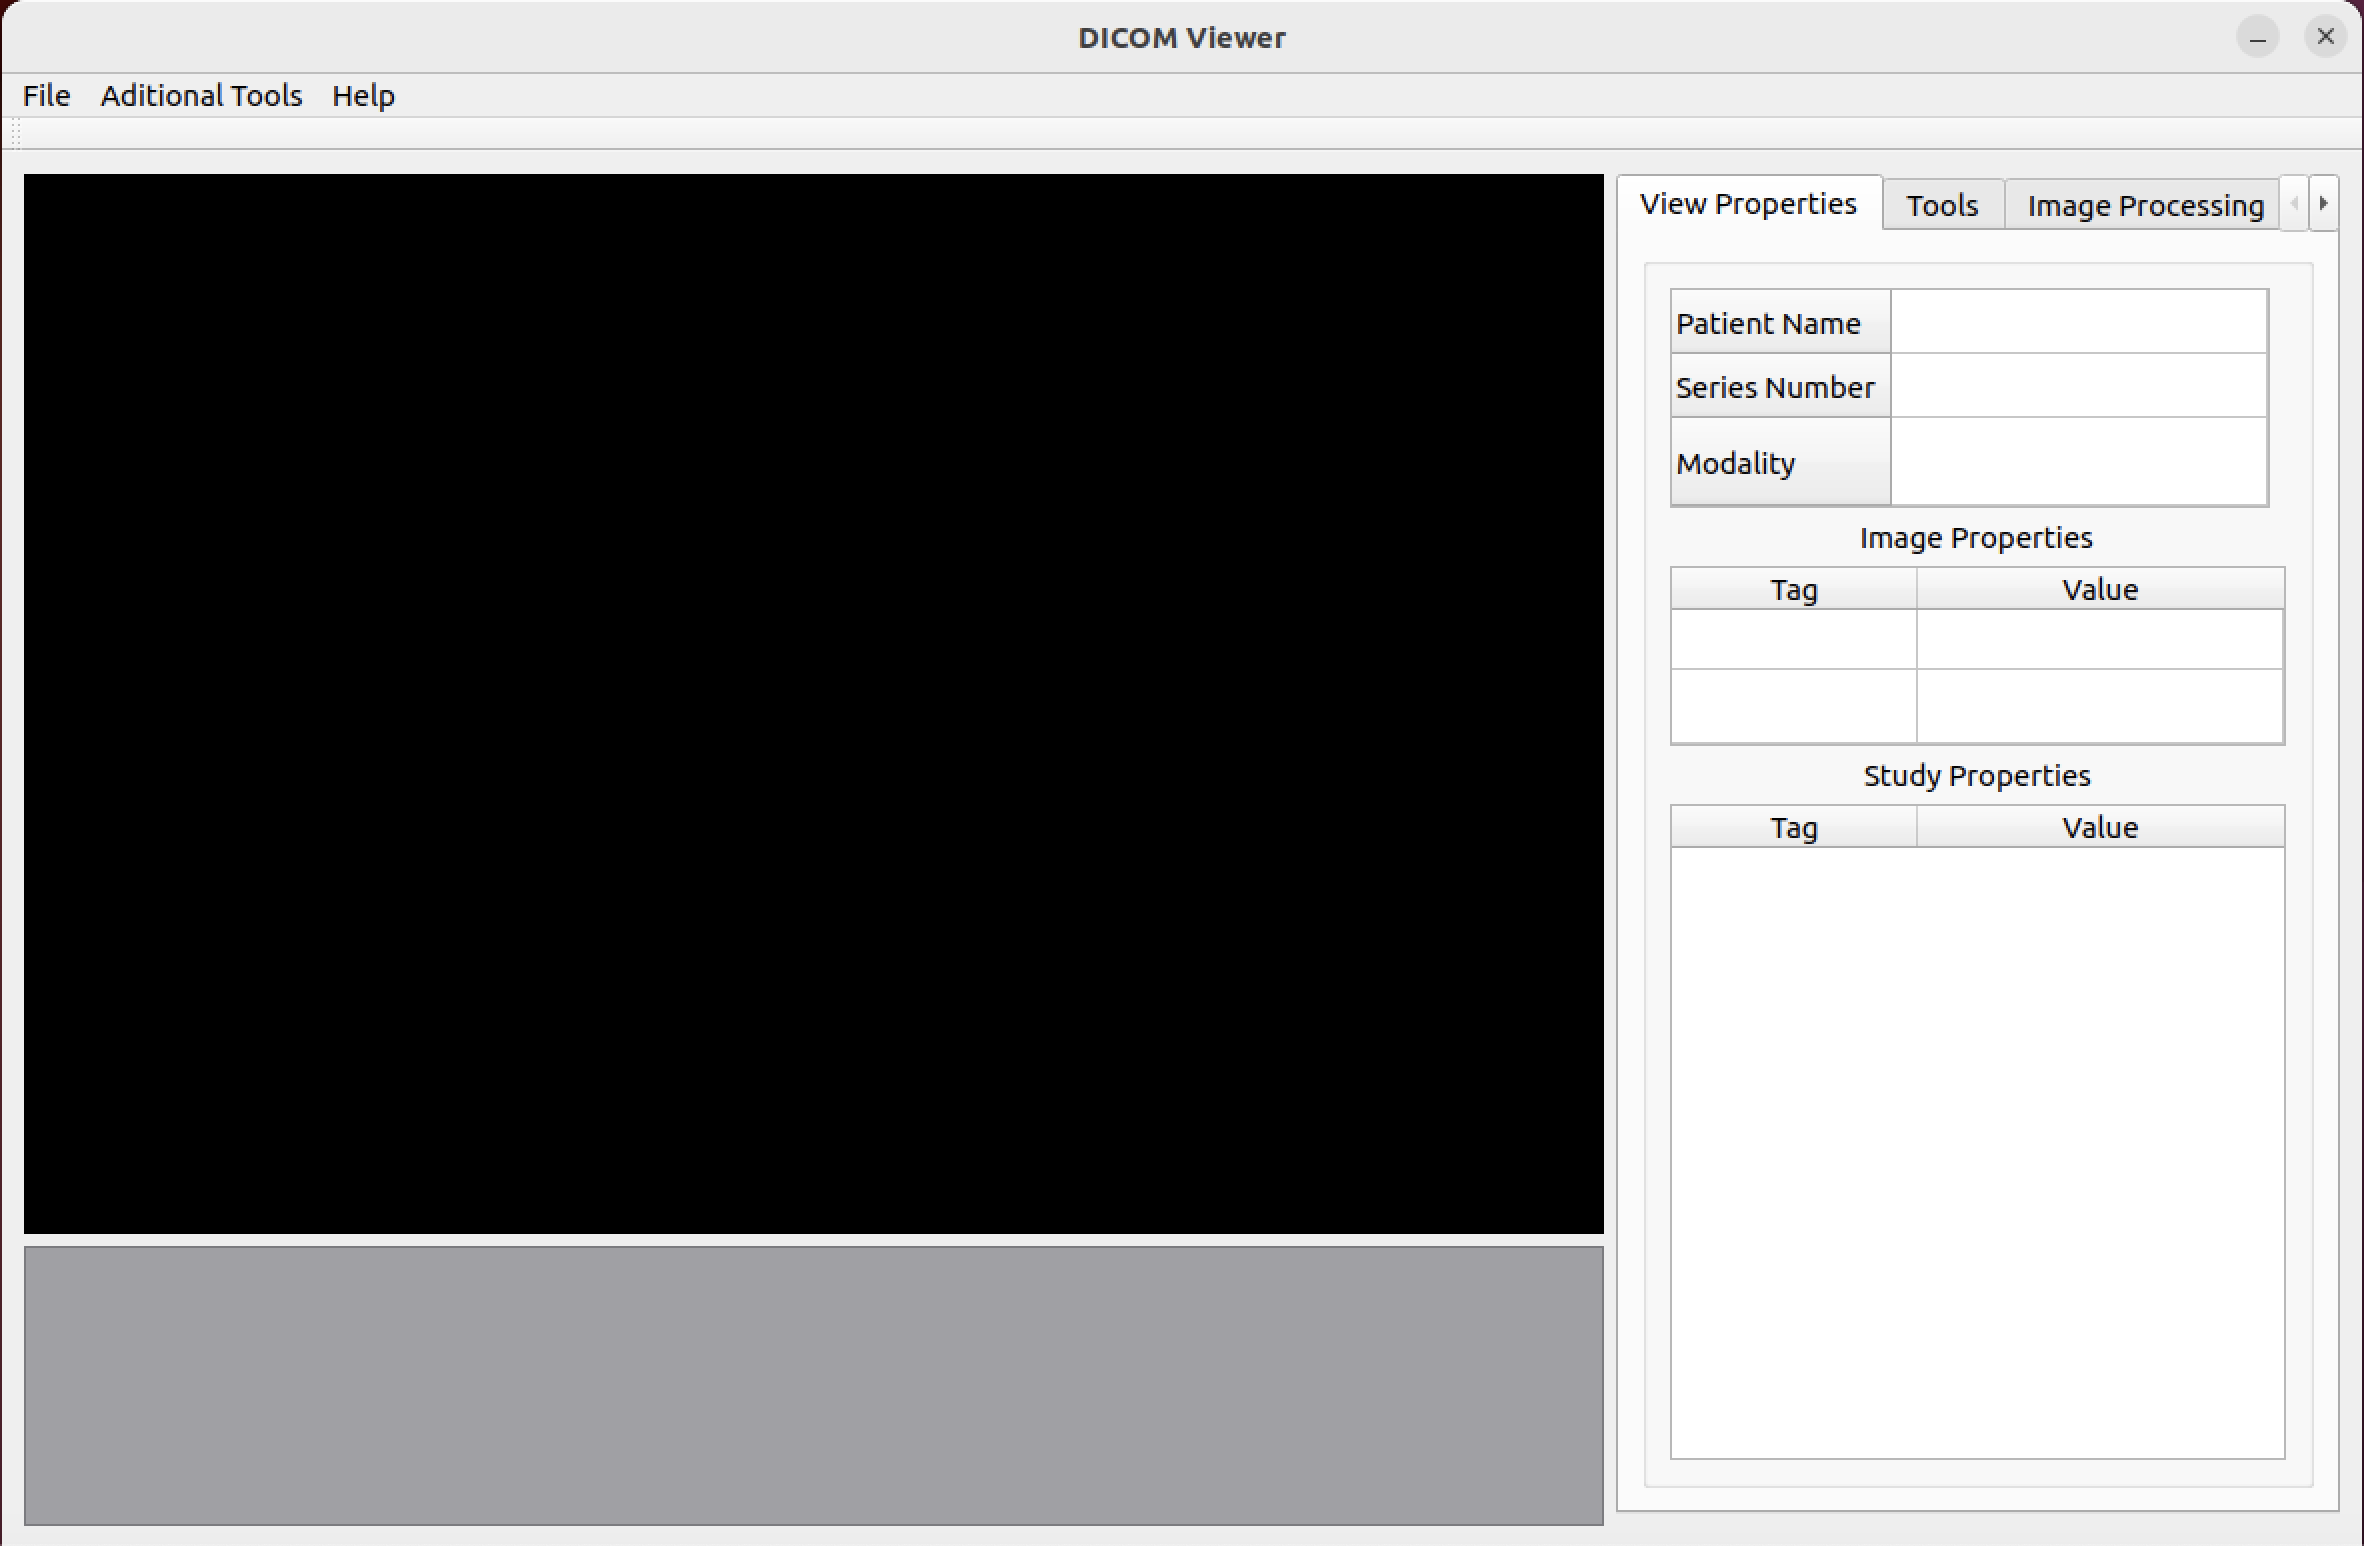
\includegraphics[height=8cm]{media/existing_app/init.png}
        \captionsetup{justification=centering}
        \captionof{figure}[Ukážka DICOM Viewer aplikácie po jej spustení]{Ukážka DICOM Viewer aplikácie po jej spustení}
\end {figure}

Používateľské rozhranie aplikácie je možné rozdeliť na nasledovné časti:
\begin {itemize}
\item {aplikačné menu,}
\item {ľavý postranný panel,}
\item {centrálnu časť aplikácie a}
\item {pravý postranný panel.}
\end {itemize}

Na zobrazenom obrázku nie je možné vidieť ľavý postranný panel, nakoľko ten je po spustení aplikácie predvolene skrytý.\clearpage

\subsection {Aplikačné menu}
V hornej časti okna aplikácie je zobrazené aplikačné menu. Toto menu pozostáva z troch hlavných možností, ktoré obsahujú viacero úrovní.

Jeho obsah je nasledovný:
\begin {enumerate}
\item {File}
	\begin {enumerate}
		\item {Open -- otvorí systémové okno pre výber priečinku s DICOM snímkami, ktoré sa majú importovať do aplikácie.}
		\item {Save Image}
		\begin {enumerate}
			\item {Save View -- uloží pohľad na aktuálnu snímku vo zvolenom formáte,}
			\item {Save Scene -- uloží scénu vo zvolenom formáte,}
			\item {Save Area of Interes [sic] -- uloží plochu záujmu vo zvolenom formáte.}
		\end {enumerate}
	\item {Save all selected}
		\begin {enumerate}
			\item {Save View -- uloží pohľad vybraných snímky vo zvolenom formáte,}
			\item {Save Scene -- uloží scénu vybraných snímkov vo zvolenom formáte,}
			\item {Save Area of Interes [sic] -- uloží plochu záujmu vybraných snímkov vo zvolenom formáte.}
		\end {enumerate}	
	\item {Exit -- ukončí aplikáciu.}
	\end {enumerate}
\item {Aditional [sic] Tools}
	\begin {enumerate}
	\item {Grid Tools -- otvorí ľavý postranný panel aplikácie s nastavením mriežky,}
	\item {Lvf Tools -- otvorí ľavý postranný panel aplikácie s nastavením filtru lokálnej variácie,}
	\item {Graph Cuts Tools -- otvorí ľavý postranný panel aplikácie s nastavením grafových rezov.}
	\end {enumerate}
\item {Help}
	\begin {enumerate}
	\item {About -- zobrazí informácie o DICOM Viewer aplikácii.}
	\end {enumerate}
\end {enumerate}

\clearpage
\subsection {Import DICOM snímiek}
Aplikácia sa po spustení nachádza v stave, v ktorom nie je možné s ňou interagovať. To je spôsobené tým, že do aplikácie je potrebné importovať aspoň jednu snímku v DICOM formáte.

Import snímiek je možné dosiahnuť zvolením možnosti File $\rightarrow{  Open}$ z aplikačného menu. Následne sa otvorí systémové okno pre výber priečinka s DICOM snímkami, ktoré sa majú zobraziť v aplikácii. Bohužiaľ nie je možné zvoliť snímky jednotlivo z priečinku, čoho dôsledkom je načítanie všetkých snímiek z vybraného priečinku do aplikácie. Po jeho zvolení sa v aplikácii zobrazí prvá importovaná snímka.

Po výbere ľubovoľnej možnosti, ktoré ponúka Aditional [sic] Tools menu, sa taktiež zobrazí ľavý postranný panel v aplikácii, ako je možné vidieť na nasledujúcej snímke aplikácie. V tomto prípade bola zvolená možnosť \uv{Grid Tools}.

\begin {figure}[ht]
        \centering
        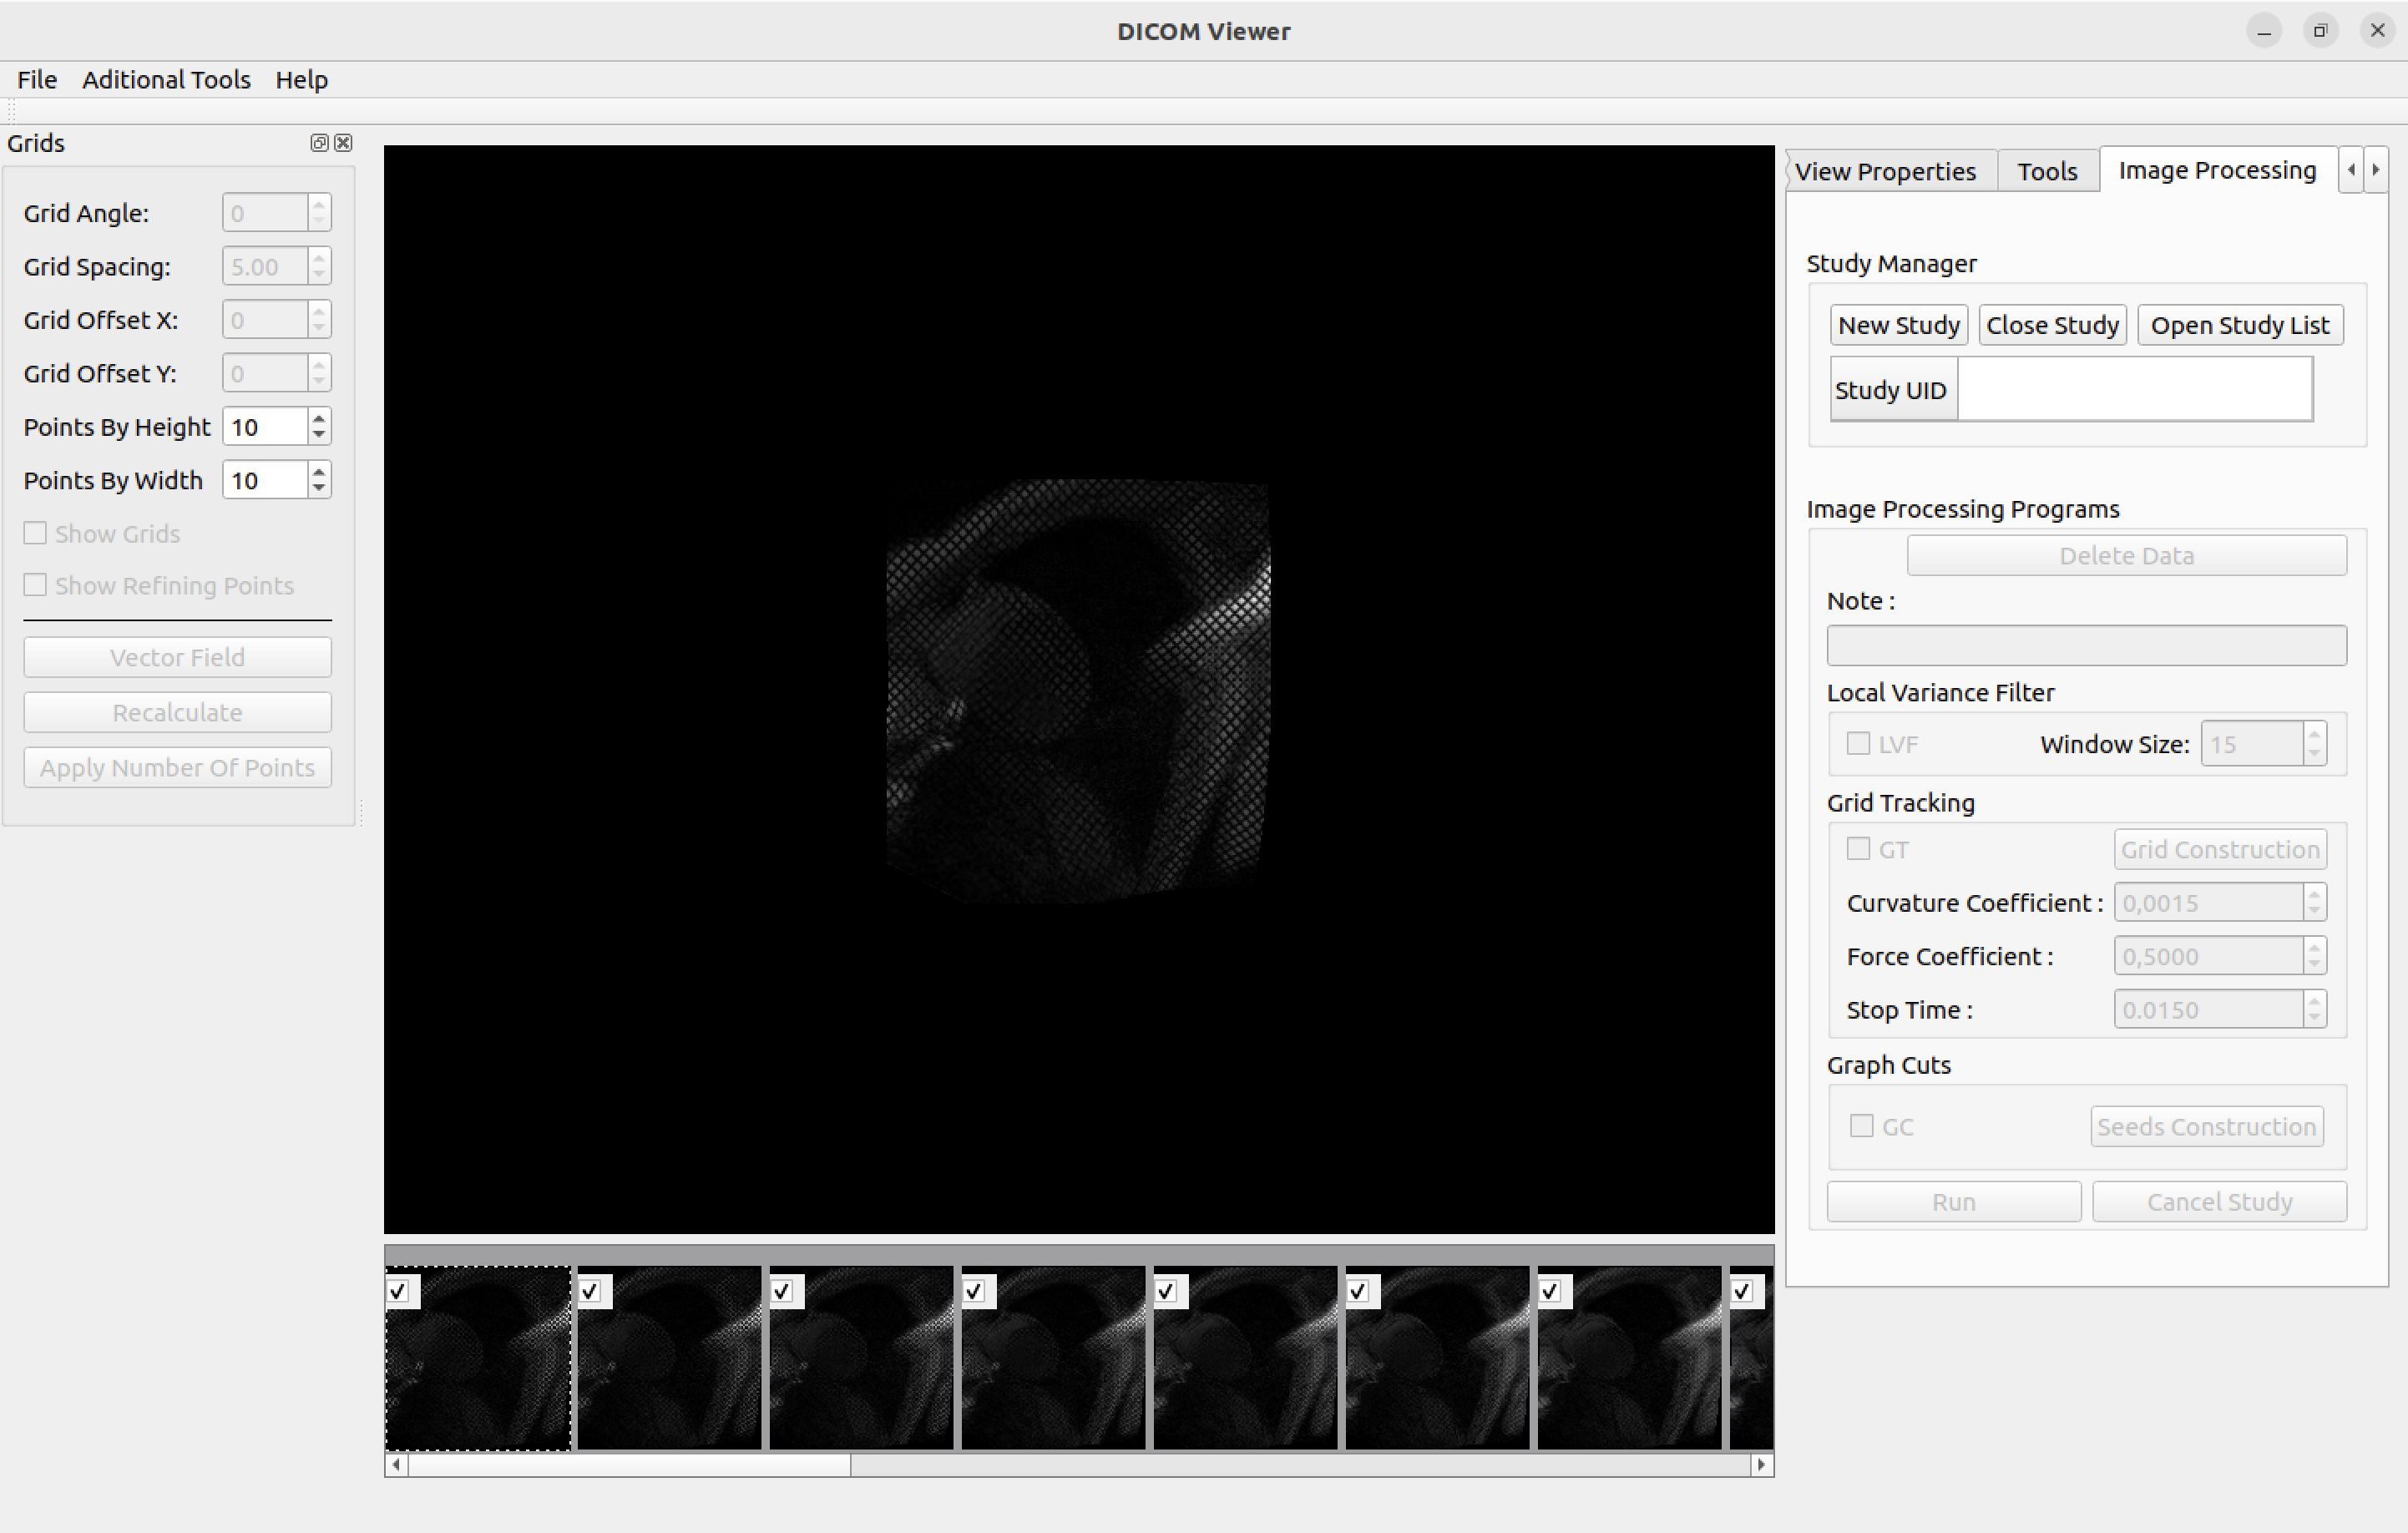
\includegraphics[height=8cm]{media/existing_app/app_with_grids_panel.png}
        \captionsetup{justification=centering}
        \captionof{figure}[Zobrazenie prvej snímky v DICOM Viewer aplikácii]{Zobrazenie prvej snímky v DICOM Viewer aplikácii}
\end {figure}

Zobrazením ľavého postranného panelu sa odhalí celková štruktúra používateľského rozhrania aplikácie.

\clearpage

\subsection {Ľavý postranný panel}\label{left_sidebar}
Obsah ľavého postranného panelu sa mení v závislosti na zvolenej možnosti\newline z menu Aditional [sic] Tools. Momentálne je na snímke zobrazený obsah ľavého panelu po zvolení možnosti \uv{Grid Tools}.

V ňom je možné nájsť nasledujúce možnosti:
\begin {itemize}
\item {Grid Angle -- uhol mriežky,}
\item {Grid Spacing -- rozpätie jednotlivých bodov,}
\item {Grid Offset X -- $x$ pozícia od ľavého horného bodu,}
\item {Grid Offset Y -- invertovaná $y$ pozícia od ľavého horného bodu,}
\item {Points by Height -- počet bodov na úsečku mriežky na výšku,}
\item {Points By Width -- počet bodov na úsečku mriežky na šírku,}
\item {Show Grids -- indikuje, či má byť zobrazená mriežka,}
\item {Show Refining Points -- indikuje, či majú byť zobrazené body, ktoré upresňujú pozíciu mriežky,}
\item {Vector Field -- spočíta rozdiel v pohybe mriežky medzi predchádzajúcou a aktuálnou snímkou,}
\item {Recalculate -- odošle dáta \texttt{grid-tracker} podprogramu pre opätovné zarovnanie mriežky voči SPAMM mriežke a}
\item {Apply Number of Points -- uloží mriežku ako textový TNL multivektor.}
\end {itemize}

Ostatné dve možnosti z menu \uv{Aditional [sic] Tools} nie je potrebné pre účely tejto práce popisovať.

\clearpage

\subsection {Centrálna plocha aplikácie}
Obsahom centrálnej plochy, ktorá je dominantná v zobrazení aplikácie, je aktuálne vybraná DICOM snímka. Nad ňou môže byť tiež vykreslená používateľom definovaná mriežka.

Pod touto plochou sú zobrazené náhľady všetkých snímiek, ktoré obsahujú zaškrtávacie políčko. Toto políčko reprezentuje možnosť, či má byť daná snímka spracovaná v rámci vybraného podprogramu.

\subsection {Pravý postranný panel}
Pravý postranný panel je rozdelený na nasledovné karty: \uv{View Properties}, \uv{Tools}, \uv{Image Processing} a \uv{History}.

\subsubsection {View Properties karta}
Karta \uv{View Properties} nie je interaktívna -- zobrazuje informácie ako meno pacienta nachádzajúceho sa na zobrazenej snímke, číslo série a modalitu snímiek. Taktiež je zobrazená výška a šírka aktuálne zobrazenej snímky.

\begin {figure}[H]
        \centering
        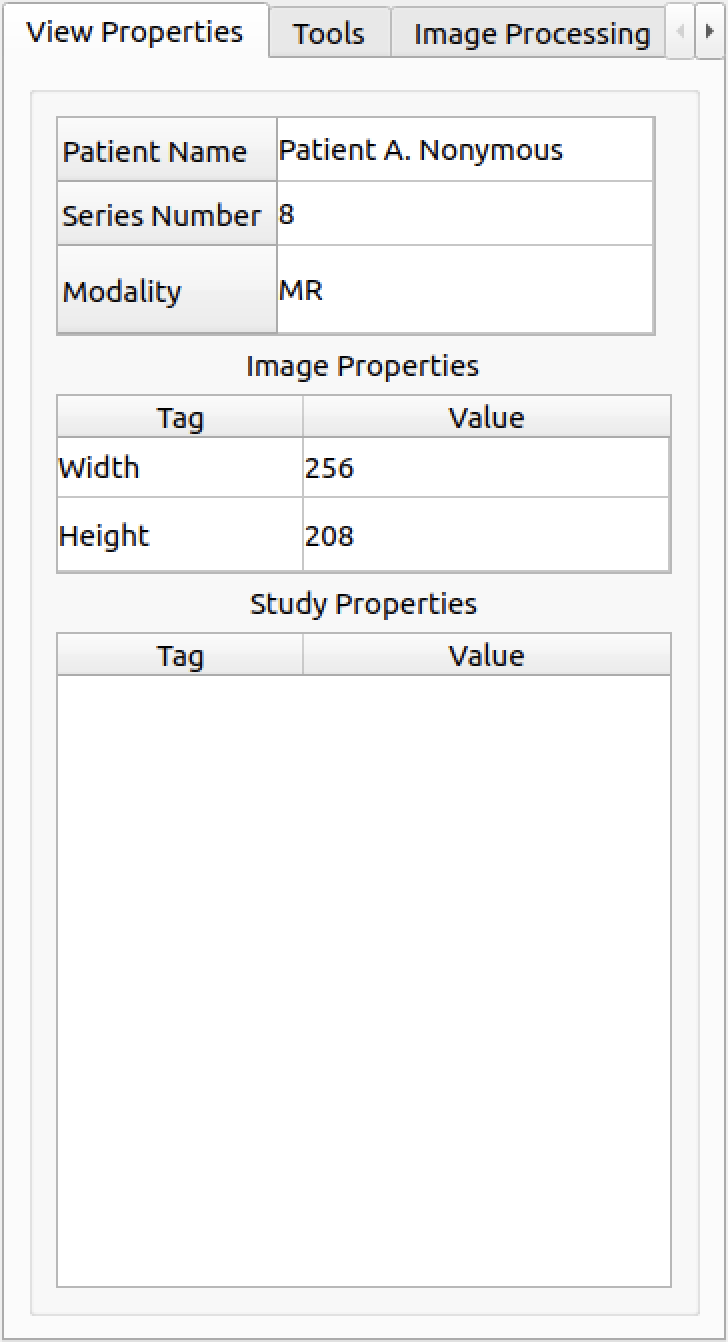
\includegraphics[height=8cm]{media/existing_app/tabs/view_properties.png}
        \captionsetup{justification=centering}
        \captionof{figure}{Zobrazenie obsahu kariet pravého postranného panelu}
\end {figure}

\clearpage

\subsubsection {Tools karta}
Narozdiel od predchádzajúcej karty, \uv{Tools} karta obsahuje interaktívne prvky, ako napr. zobrazenie a zmena indexu zobrazenej snímky, či slider pre jej priblíženie. Snímke je taktiež možné zmeniť kontrast, jas a gammu pomocou sliderov.

Ďalej nasleduje sekcia pre nastavenie oblasti záujmu, pri ktorej je možné nastaviť jej zobrazenie alebo zmeniť jej výšku/šírku -- oblasť záujmu je na základe týchto nastavení vykreslená nad snímkou. 

Keďže aplikácia podporuje animáciu snímiek, je možné nastaviť jej rýchlosť v milisekundách (čo predstavuje čas, v rámci ktorého bude zobrazená jedna snímka), nastavenie počiatočnej snímky, od ktorej sa animácia spustí a poslednej snímky, po ktorú animácia bude spustená. Okrem nastavenia parametrov animácie nesmú chýbať tlačidlá pre spustenie a zastavenie animácie.

\begin {figure}[H]
        \centering
        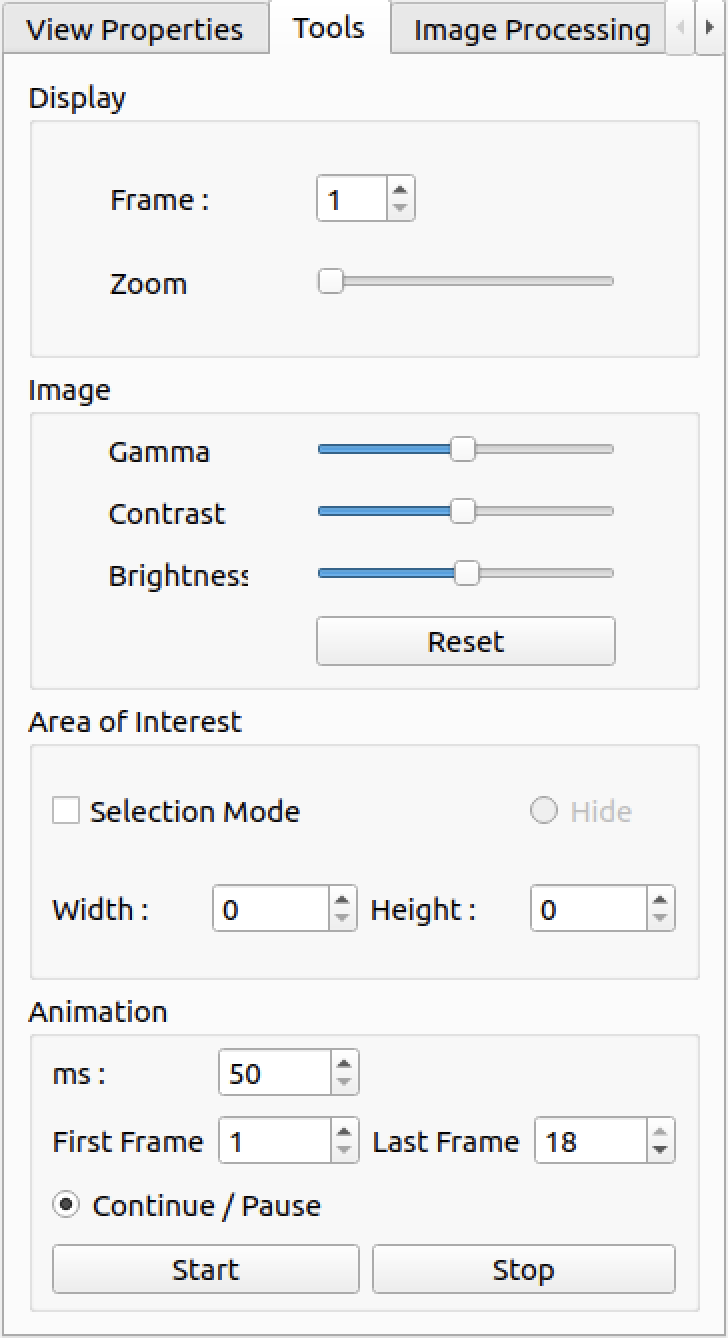
\includegraphics[height=8cm]{media/existing_app/tabs/tools.png}
        \captionsetup{justification=centering}
        \captionof{figure}{Zobrazenie obsahu kariet pravého postranného panelu}
\end {figure}

\clearpage

\subsubsection {Image Processing karta}\label{image_processing_tab}
Na \uv{Image Processing} karte sa nachádzajú tlačidlá ovládajúce manažéra štúdií. Jeho úlohou je zoskupovať rôzne štúdie, v rámci ktorých sa ukladajú parametre jej konfigurácie. Po kliknutí na tlačidlo \uv{Open Study List} sa zobrazí nové okno so všetkými štúdiami a ich parametrami. Pre interakciu s ostatnými poliami na tejto karte je potrebné najprv vytvoriť novú štúdiu kliknutím\newline na tlačidlo \uv{New Study}. Štúdiu je tiež možné ukončiť zvolením tlačidla\newline \uv{Close Study}. Každá štúdia je reprezentovaná jedinečným ID, ktoré sa skladá z dátumu a času jej vytvorenia.

Vytvorením novej štúdie sa aktivujú polia \uv{Image Processing Programs} sekcie. Táto sekcia ponúka tri hlavné zaškrtávacie políčka -- prvé reprezentuje aplikáciu filtra lokálnej variancie. Druhé z nich reprezentuje spustenie algoritmu pre zarovnanie vygenerovanej mriežky s mriežkou myokardu vytvorenou pomocou SPAMM techniky a tretie spustenie algoritmu segmentácie srdečných komôr pomocou grafových rezov. Zaškrtnutím daného políčka a kliknutím na tlačidlo \uv{Run} sa spustí algoritmus príslušný danému políčku. Pre \uv{Grid Tracking} algoritmus je v tejto sekcii možné definovať tri parametre, a to \uv{Curvature Coefficient}, \uv{Force Coefficient} a \uv{Stop Time} (viď \ref{helper_apps}).

\begin {figure}[H]
        \centering
        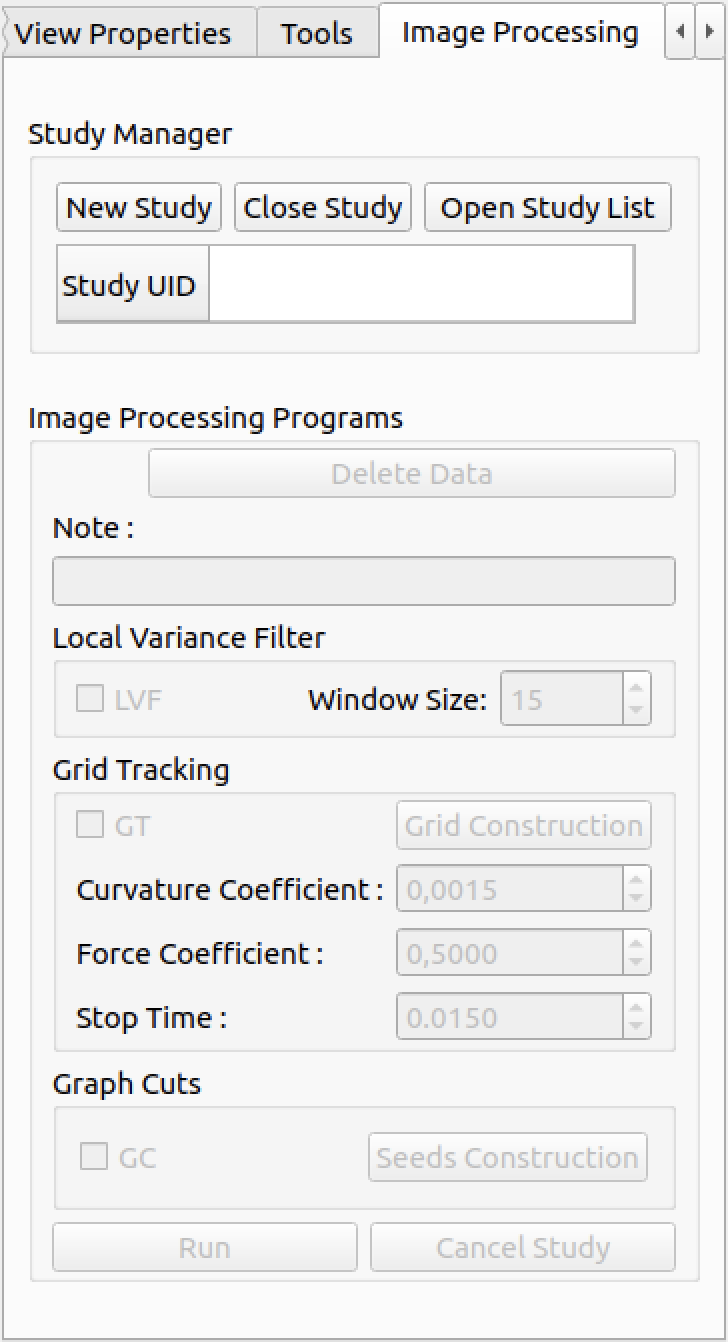
\includegraphics[height=8cm]{media/existing_app/tabs/image_processing_inactive.png}
        \captionsetup{justification=centering}
        \captionof{figure}{Zobrazenie obsahu kariet pravého postranného panelu}
\end {figure}

\subsubsection {History karta}
Účelom poslednej karty \uv{History} je výpis rozličných záznamov pre informovanie používateľa o prebiehajúcich krokoch aplikácie.

\begin {figure}[H]
        \centering
        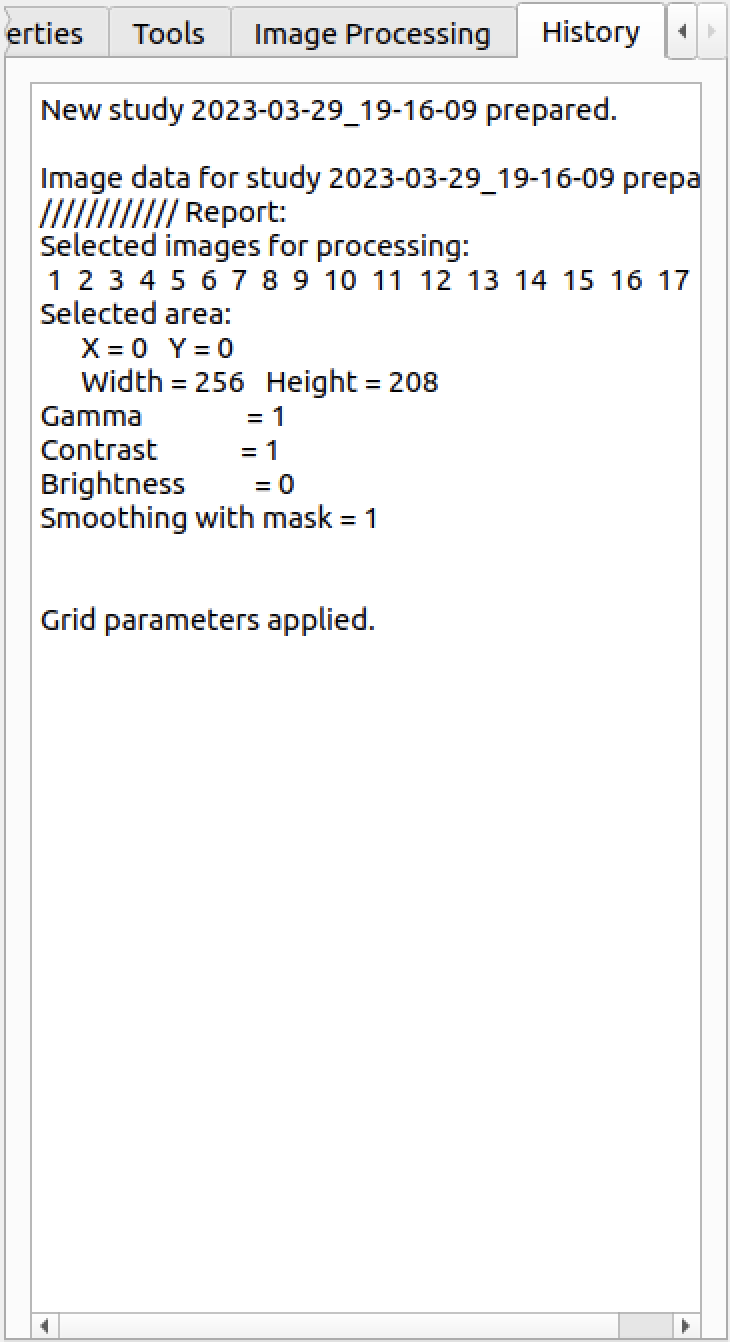
\includegraphics[height=8cm]{media/existing_app/tabs/history.png}
        \captionsetup{justification=centering}
        \captionof{figure}{Zobrazenie obsahu kariet pravého postranného panelu}
\end {figure}

\section {Testovanie a návrhy pre webovú aplikáciu}
Účelom testovania súčasnej aplikácie je zoznámenie sa s aplikáciou a jej procesmi, ako aj overenie jej funkcionality a zistenia používateľského zážitku.

Počas samotného testovania bolo možné úspešne importovať DICOM súbory a zobraziť ich snímky. Snímky bolo taktiež možné animovať na základe nastavenia animácie, zmeniť im kontrast a jas, či ich priblížiť alebo oddialiť.

Následne bola odtestovaná funkcionalita týkajúca sa vykreslenia mriežky a jej úprav. Vykreslenie mriežky prebehlo bezchybne -- avšak jej počiatočná poloha bola vždy fixne určená v ľavom hornom okraji snímky.

\clearpage

Toto správanie by sa dalo navrhnúť tak, aby bolo možné určiť počiatočné koordináty vytváranej mriežky jednoduchým kliknutím myši na miesto, kde by mala byť mriežka vykreslená.

Pri priblížení vykreslenej mriežky absentuje posun snímky samotným potiahnutím myši -- posun snímky na ploche bolo možné len pomocou scrollbarov, ktoré boli ťažkopádnejšie na ovládanie.

Taktiež úprava polohy mriežky bola možná len pomocou stlačenia klávesy \texttt{Shift} a potiahnutím myši. Tento spôsob posunu avšak nie je používateľovi nikde odprezentovaný. Návrh používateľského rozhrania webovej aplikácie by mal preto uľahčiť prípadnú zmenu polohy snímky na ploche.

\subsection {Problémy s \texttt{grid-tracker} podprogramom}\label{grid_tracker_issues}
Po úprave polohy mriežky nasledovalo spustenie samotného výpočtu zodpovedného za určenie súradníc bodov mriežok tak, aby zodpovedali vytvorenej mriežke pomocou SPAMM technológie. Pri spustení tohto algoritmu avšak aplikácia spadla. Nasledoval debugging aplikácie, ktorý potvrdil, že daný algoritmus nebol dokončený a prepojený so súčasnou aplikáciou.

Školiteľ bol následne s týmto problémom oboznámený. Po vzájomnej diskusii vzišlo k nasledujúcej dohode -- možnosti prepojenia \texttt{grid-tracker} podprogramu s webovou aplikáciou budú zanalyzované a výsledné prepojenie navrhnuté, avšak následná implementácia prepojenia s týmto podprogramom sa neuskutoční, nakoľko jeho algoritmus bude potrebné upraviť tak aby nielen správne fungoval, ale navyše bol kompatibilný s najnovšou verziou TNL knižnice.

Webová aplikácia bude naďalej prijímať dáta potrebné pre samotný výpočet a odosielať výstup v štruktúrovanej podobe, avšak ten bude do určitej podoby reflektovať prijaté dáta, keďže dané prepojenie s \texttt{grid-tracker} podprogramom nebude implementované. Tento proces prijatia dát, výpočtu a ich odoslanie bude v nasledujúcich častiach spomínaný pod pojmom \uv{SPAMM algoritmus}.